% Rapport PFE EMSI - Shopify Price Intelligence
% Compiler avec LuaLaTeX puis BibTeX: voir README.md.
\documentclass[12pt,a4paper,oneside]{report}

% ----- Langues et typographie -----
\usepackage{fontspec}
\usepackage[main=french,english,arabic]{babel}
\babelfont{rm}{Latin Modern Roman}
\babelfont[arabic]{rm}{Amiri}
\usepackage{microtype}
\usepackage{setspace}
\onehalfspacing

% ----- Mise en page imposee par le guide EMSI -----
\usepackage{geometry}
\geometry{top=2.5cm,bottom=2.5cm,left=3cm,right=2.5cm}
\usepackage{fancyhdr}
\usepackage{titlesec}
\usepackage{tocloft}
\usepackage{graphicx}
\graphicspath{{../}}
\usepackage{float}
\usepackage{caption}
\usepackage{booktabs}
\usepackage{longtable}
\usepackage{tabularx}
\usepackage{array}
\usepackage{multirow}
\usepackage{xcolor}
\usepackage{listings}
\usepackage{amsmath,amssymb}
\usepackage{tikz}
\usetikzlibrary{arrows.meta,positioning,shapes.geometric,fit}
\usepackage{enumitem}
\usepackage{hyperref}
\usepackage{url}

\hypersetup{
  colorlinks=true,
  linkcolor=black,
  citecolor=black,
  urlcolor=blue!55!black,
  pdftitle={Rapport PFE - Shopify Price Intelligence},
  pdfauthor={A completer}
}

\definecolor{emsiBlue}{HTML}{123C69}
\definecolor{softBlue}{HTML}{EAF2F8}
\definecolor{codeGray}{HTML}{F4F6F7}
\definecolor{placeholderRed}{HTML}{A61B1B}

\titleformat{\chapter}[display]
  {\normalfont\fontsize{16}{19}\selectfont\bfseries\color{emsiBlue}}
  {\chaptername\ \thechapter}{0.4em}{\centering}
\titleformat{\section}
  {\normalfont\fontsize{14}{17}\selectfont\bfseries\color{emsiBlue}}
  {\thesection}{0.75em}{}
\titleformat{\subsection}
  {\normalfont\fontsize{12}{14}\selectfont\bfseries}
  {\thesubsection}{0.75em}{}
\titlespacing*{\chapter}{0pt}{0pt}{20pt}
\titlespacing*{\section}{0pt}{18pt}{8pt}
\titlespacing*{\subsection}{0pt}{12pt}{6pt}

\captionsetup{font=small,labelfont=bf}
\setlist[itemize]{leftmargin=1.2cm,itemsep=3pt,topsep=4pt}
\setlist[enumerate]{leftmargin=1.2cm,itemsep=3pt,topsep=4pt}
\renewcommand{\arraystretch}{1.25}
\newcolumntype{Y}{>{\raggedright\arraybackslash}X}

\lstdefinestyle{typescript}{
  language=JavaScript,
  basicstyle=\small\ttfamily,
  backgroundcolor=\color{codeGray},
  frame=single,
  rulecolor=\color{black!15},
  breaklines=true,
  columns=fullflexible,
  keywordstyle=\color{blue!60!black}\bfseries,
  commentstyle=\color{green!40!black},
  stringstyle=\color{red!55!black},
  showstringspaces=false,
  captionpos=b
}

\pagestyle{fancy}
\fancyhf{}
\fancyhead[L]{\small Shopify Price Intelligence}
\fancyhead[R]{\small Rapport de PFE}
\fancyfoot[C]{\thepage}
\renewcommand{\headrulewidth}{0.4pt}
\renewcommand{\footrulewidth}{0pt}

% ----- Metadonnees a completer avant soumission -----
\newcommand{\studentName}{\textcolor{placeholderRed}{[Nom et prenom de l'etudiant]}}
\newcommand{\programName}{\textcolor{placeholderRed}{[Filiere d'ingenierie]}}
\newcommand{\academicAdvisor}{\textcolor{placeholderRed}{[Nom de l'encadrant academique]}}
\newcommand{\industryAdvisor}{\textcolor{placeholderRed}{[Nom de l'encadrant industriel]}}
\newcommand{\hostCompany}{\textcolor{placeholderRed}{[Nom de l'entreprise d'accueil]}}
\newcommand{\academicYear}{2025--2026}
\newcommand{\reportTitle}{Conception et realisation d'une plateforme d'intelligence tarifaire pour les marchands Shopify}
\newif\ifdedication
\dedicationfalse % Passer a \dedicationtrue pour afficher la dedicace optionnelle.

\begin{document}

% ==================== Page de garde ====================
\begin{titlepage}
  \thispagestyle{empty}
  \begin{center}
    \begin{minipage}[t]{0.38\textwidth}
      \centering
      \fbox{\parbox[c][2.1cm][c]{0.8\textwidth}{\centering\bfseries Logo EMSI\\\small A inserer}}
    \end{minipage}
    \hfill
    \begin{minipage}[t]{0.38\textwidth}
      \centering
      \fbox{\parbox[c][2.1cm][c]{0.8\textwidth}{\centering\bfseries Logo entreprise\\\small A inserer}}
    \end{minipage}

    \vspace{1.2cm}
    {\Large\bfseries Ecole Marocaine des Sciences de l'Ingenieur\\[0.15cm]}
    {\large Centre EMSI Rabat\\[0.5cm]}
    {\large \programName\par}

    \vfill
    {\fontsize{18}{22}\selectfont\bfseries RAPPORT DE PROJET DE FIN D'ETUDES\par}
    \vspace{0.8cm}
    \rule{\textwidth}{0.8pt}\\[0.45cm]
    {\fontsize{18}{23}\selectfont\bfseries\color{emsiBlue}\reportTitle\par}
    \vspace{0.45cm}
    \rule{\textwidth}{0.8pt}
    \vfill

    \begin{tabularx}{\textwidth}{@{}Y Y@{}}
      \textbf{Realise par :} & \textbf{Encadre par :} \\
      \studentName & \academicAdvisor \\
      & \industryAdvisor \\
      \addlinespace[0.45cm]
      \textbf{Entreprise d'accueil :} & \textbf{Annee universitaire :} \\
      \hostCompany & \academicYear \\
    \end{tabularx}

    \vfill
    \textit{Soutenu publiquement devant un jury compose d'enseignants et de professionnels.}
  \end{center}
\end{titlepage}

\pagenumbering{roman}
\setcounter{page}{1}

\ifdedication
\chapter*{Dedicace}
\addcontentsline{toc}{chapter}{Dedicace}
\thispagestyle{plain}
\vspace*{5cm}
\begin{flushright}
\textit{[Dedicace personnelle a completer.]}
\end{flushright}
\clearpage
\fi

% ==================== Remerciements ====================
\chapter*{Remerciements}
\addcontentsline{toc}{chapter}{Remerciements}
\thispagestyle{plain}
Je remercie tout d'abord \hostCompany{} pour l'accueil, l'environnement de travail et les ressources mises a disposition pendant la realisation de ce projet. Je remercie particulierement \industryAdvisor{} pour son accompagnement, ses retours metier et son aide dans la clarification des besoins lies au pilotage des prix dans le commerce electronique.

J'adresse egalement mes remerciements a \academicAdvisor{} pour l'encadrement academique, la rigueur methodologique et les conseils apportes tout au long de la conception et de la realisation. Mes remerciements vont enfin a l'ensemble des enseignants de l'EMSI, ainsi qu'a toutes les personnes qui ont contribue, directement ou indirectement, a l'aboutissement de ce travail.

\clearpage

% ==================== Resumes ====================
\chapter*{Resume}
\addcontentsline{toc}{chapter}{Resume}
\thispagestyle{plain}
La fixation d'un prix competitif est une decision recurrente pour les marchands en ligne. Elle exige de suivre des produits comparables, de verifier la fiabilite des informations collectees et de preserver la marge commerciale. Or, une surveillance manuelle des sites concurrents est lente, fragile et difficile a generaliser lorsque le catalogue s'agrandit. Ce projet presente la conception et la realisation de \textit{Shopify Price Intelligence}, une plateforme web destinee aux marchands Shopify pour centraliser le suivi des prix concurrents et produire des recommandations tarifaires exploitables.

La solution repose sur une interface React, une API TypeScript basee sur Express et tRPC, et une base PostgreSQL accedee avec Drizzle ORM. Elle permet l'authentification des utilisateurs, la connexion d'une boutique Shopify, la synchronisation de produits, la gestion de concurrents, l'enregistrement d'historiques de prix et la diffusion d'alertes. Le processus de surveillance combine la collecte de pages concurrentes, une extraction assistee par IA, la verification du rapprochement produit et la detection de variations. Un moteur de recommandation calcule une position de marche et applique un sous-cotation de 5\% de la moyenne concurrentielle, tout en imposant un seuil de protection de marge lorsque le cout du produit est connu.

Le travail couvre l'analyse des besoins, la conception de l'architecture et des donnees, l'implementation des principaux modules et un protocole de validation. L'objectif est de transformer des donnees de marche dispersees en decisions tarifaires traceables, avec une attention particuliere a la securite, a la propriete des donnees et a la lisibilite de l'interface.

\noindent\textbf{Mots-cles :} Shopify, veille concurrentielle, intelligence tarifaire, recommandation de prix, commerce electronique.
\clearpage

\chapter*{Abstract}
\addcontentsline{toc}{chapter}{Abstract}
\thispagestyle{plain}
Setting a competitive price is a recurring decision for online merchants. It requires tracking comparable products, assessing the reliability of the collected information, and preserving the commercial margin. Manual monitoring of competitor websites is slow, fragile, and difficult to scale as a catalogue grows. This project presents the design and implementation of \textit{Shopify Price Intelligence}, a web platform for Shopify merchants that centralizes competitor-price monitoring and produces actionable pricing recommendations.

The solution relies on a React interface, a TypeScript API built with Express and tRPC, and a PostgreSQL database accessed through Drizzle ORM. It supports user authentication, Shopify-store connection, product synchronization, competitor management, price-history storage, and alert delivery. The monitoring process combines competitor-page collection, AI-assisted extraction, product-match verification, and price-change detection. A recommendation engine calculates a market position and applies a five-percent undercut of the competitor average while enforcing a margin-protection floor when the product cost is known.

This work covers requirements analysis, architecture and data design, implementation of the principal modules, and a validation protocol. Its purpose is to turn scattered market information into traceable pricing decisions, with particular attention to security, data ownership, and interface readability.

\noindent\textbf{Keywords:} Shopify, competitor monitoring, price intelligence, price recommendation, e-commerce.
\clearpage

\chapter*{\begin{otherlanguage}{arabic}ملخص\end{otherlanguage}}
\addcontentsline{toc}{chapter}{ملخص}
\thispagestyle{plain}
\begin{otherlanguage}{arabic}
\begin{RTL}
يعد تحديد سعر تنافسي قرارا متكررا بالنسبة للتجار عبر الإنترنت. فهو يتطلب تتبع المنتجات المماثلة، والتحقق من موثوقية المعلومات المجمعة، والحفاظ على الهامش التجاري. إن المراقبة اليدوية لمواقع المنافسين بطيئة وهشة ويصعب توسيعها مع نمو الكتالوج. يقدم هذا المشروع تصميم وإنجاز منصة \textit{Shopify Price Intelligence} الموجهة لتجار Shopify من أجل تجميع مراقبة أسعار المنافسين وإنتاج توصيات سعرية قابلة للتنفيذ.

تعتمد المنصة على واجهة React وواجهة برمجة تطبيقات TypeScript مبنية على Express وtRPC وقاعدة بيانات PostgreSQL يتم الوصول إليها عبر Drizzle ORM. تتيح المنصة المصادقة، وربط متجر Shopify، ومزامنة المنتجات، وإدارة المنافسين، وحفظ تاريخ الأسعار، وإرسال التنبيهات. تجمع عملية المراقبة بين جمع صفحات المنافسين، واستخراج المعلومات بمساعدة الذكاء الاصطناعي، والتحقق من تطابق المنتجات، واكتشاف تغيرات الأسعار. كما يحسب محرك التوصية وضع المنتج في السوق ويقترح سعرا أقل بنسبة خمسة بالمائة من متوسط أسعار المنافسين مع احترام حد أدنى لحماية الهامش عند توفر تكلفة المنتج.
\end{RTL}
\end{otherlanguage}
\clearpage

% ==================== Tables automatiques ====================
\tableofcontents
\clearpage
\addcontentsline{toc}{chapter}{Liste des figures}
\listoffigures
\clearpage
\addcontentsline{toc}{chapter}{Liste des tableaux}
\listoftables
\clearpage

\chapter*{Liste des abreviations et acronymes}
\addcontentsline{toc}{chapter}{Liste des abreviations et acronymes}
\begin{longtable}{p{0.22\textwidth}p{0.7\textwidth}}
\toprule
\textbf{Acronyme} & \textbf{Signification} \\
\midrule
\endhead
API & Application Programming Interface \\
CSRF & Cross-Site Request Forgery \\
HMAC & Hash-based Message Authentication Code \\
IA & Intelligence Artificielle \\
JWT & JSON Web Token \\
ORM & Object-Relational Mapping \\
PFE & Projet de Fin d'Etudes \\
SSE & Server-Sent Events \\
tRPC & TypeScript Remote Procedure Call \\
UI & User Interface \\
\bottomrule
\end{longtable}
\clearpage

\pagenumbering{arabic}
\setcounter{page}{1}

% ==================== Introduction generale ====================
\chapter*{Introduction generale}
\addcontentsline{toc}{chapter}{Introduction generale}
\markboth{Introduction generale}{Introduction generale}

Le commerce electronique evolue dans un environnement ou les prix, les promotions et la disponibilite des produits peuvent changer rapidement. Pour un marchand Shopify, la connaissance du marche est indispensable, mais elle est rarement disponible sous une forme directement exploitable. Les informations sont reparties entre le catalogue de la boutique, les fiches de concurrents et les canaux de vente externes. Le suivi manuel de ces donnees conduit a des decisions tardives et peu traceables.

La problematique traitee est donc la suivante : \textit{comment fournir a un marchand Shopify une vision fiable et actionnable de sa position tarifaire, tout en preservant ses contraintes de marge et la securite de ses donnees ?} La reponse proposee est une plateforme d'intelligence tarifaire qui importe les produits d'une boutique, observe des offres concurrentes, historise les donnees et formule une recommandation explicable.

Les objectifs du projet sont les suivants :
\begin{itemize}
  \item automatiser la collecte et l'organisation des informations tarifaires pertinentes ;
  \item assister le rapprochement entre un produit interne et une offre concurrente ;
  \item detecter les variations importantes et notifier le marchand ;
  \item proposer un prix cible qui tient compte du marche et d'un seuil minimal de marge ;
  \item proposer une application securisee, multi-utilisateur et lisible.
\end{itemize}

La demarche adoptee combine une analyse des besoins, une conception par couches, une implementation TypeScript de bout en bout et la definition de tests fonctionnels et unitaires. Le premier chapitre presente le contexte et les besoins. Le deuxieme decrit les specifications et les choix de conception. Le troisieme detaille l'architecture, les donnees et l'algorithme tarifaire. Le quatrieme expose la realisation, la strategie de validation et les limites identifiees.
\clearpage

% ==================== Chapitre 1 ====================
\chapter{Contexte general et analyse des besoins}
\section*{Introduction du chapitre}
Ce chapitre situe le projet dans son contexte metier, identifie les parties prenantes et formalise le besoin auquel la plateforme repond.

\section{Contexte du projet}
Les petites equipes e-commerce doivent concilier acquisition, logistique, relation client et gestion du catalogue. Le controle continu des prix concurrents devient alors une tache repetitive qui consomme du temps sans toujours fournir une decision claire. Un prix trop eleve peut reduire la competitivite d'une offre, tandis qu'une baisse non controlee peut detruire la marge. L'enjeu n'est donc pas simplement de trouver le prix le plus bas, mais de fournir une information contextualisee permettant au marchand de choisir.

La plateforme cible les marchands Shopify et les petites equipes responsables d'un catalogue. Son principe directeur est de reduire le temps entre l'observation d'un changement de marche et une action documentee. Le produit vise une experience concise : le marchand doit identifier les produits qui requierent son attention, comprendre la recommandation et retrouver les donnees qui la justifient.

\section{Parties prenantes et acteurs}
\begin{table}[H]
\centering
\caption{Acteurs principaux et responsabilites}
\label{tab:actors}
\begin{tabularx}{\textwidth}{p{0.22\textwidth}Y Y}
\toprule
\textbf{Acteur} & \textbf{Attentes} & \textbf{Interactions avec la plateforme} \\
\midrule
Marchand Shopify & Connaitre sa position tarifaire et agir rapidement. & Connecte sa boutique, consulte les produits, les alertes et les recommandations. \\
Equipe e-commerce & Superviser plusieurs produits et conserver une trace des changements. & Gere le catalogue, les concurrents et les preferences de notification. \\
Administrateur & Maintenir un usage controle de la plateforme. & Administre les comptes et supervise les operations necessaires. \\
Shopify & Autoriser l'acces aux donnees de boutique selon des permissions explicites. & Fournit le flux d'autorisation et les donnees de produits. \\
Services externes & Rendre les pages concurrentes exploitables. & Participent a la recherche, au scraping et a l'extraction structuree. \\
\bottomrule
\end{tabularx}
\end{table}

\section{Problematique et objectifs}
La problematique se decompose en quatre difficultes. La premiere est l'heterogeneite des sources : les donnees de prix n'ont pas toujours la meme structure ni le meme niveau de qualite. La deuxieme est le rapprochement : une offre trouvee ne correspond pas necessairement au meme produit, modele ou variante. La troisieme est la frequence : les prix evoluent et doivent etre historises plutot qu'ecrases. La quatrieme est la decision : une recommandation doit rester compatible avec le cout du produit et etre explicable.

L'objectif general consiste a concevoir une chaine coherente allant de la synchronisation du catalogue jusqu'a l'alerte ou a la recommandation. Les objectifs techniques associes sont la separation des responsabilites entre interface, API, services et persistance ; l'isolation des donnees de chaque utilisateur ; la protection des secrets d'integration ; et la conservation d'un historique permettant l'analyse.

\section{Expression des besoins fonctionnels}
\begin{table}[H]
\centering
\caption{Exigences fonctionnelles principales}
\label{tab:functional-requirements}
\begin{tabularx}{\textwidth}{p{0.12\textwidth}p{0.34\textwidth}Y}
\toprule
\textbf{ID} & \textbf{Exigence} & \textbf{Critere d'acceptation} \\
\midrule
F01 & Authentifier un utilisateur et proteger les ecrans prives. & Un utilisateur non authentifie est redirige vers l'ecran de connexion. \\
F02 & Connecter une boutique Shopify. & Le marchand autorise l'application et voit sa boutique active dans les parametres. \\
F03 & Synchroniser les produits de la boutique. & Les produits importes sont rattaches au compte et a la boutique concernee. \\
F04 & Gerer les concurrents et les produits concurrents. & Le marchand peut consulter, ajouter ou suivre des offres concurrentes. \\
F05 & Historiser les observations de prix. & Chaque collecte pertinente cree un instantane reutilisable pour l'analyse. \\
F06 & Detecter un changement et produire une alerte. & Une variation significative cree un evenement et une notification. \\
F07 & Produire une recommandation de prix. & La recommandation affiche le contexte de marche et le seuil de protection applique. \\
F08 & Rechercher les produits et concurrents. & Les resultats sont limites au perimetre de l'utilisateur connecte. \\
\bottomrule
\end{tabularx}
\end{table}

\section{Exigences non fonctionnelles}
La securite est essentielle car l'application manipule des comptes utilisateurs et des jetons permettant d'acceder a Shopify. Les acces doivent etre controles, les donnees sensibles stockees de maniere chiffree et les operations exposees protegees contre les abus. Les controles implementes s'inscrivent dans une demarche de reduction des risques courants d'applications web, notamment l'authentification, le controle d'acces, la cryptographie et la journalisation \cite{owasp2025}.

La qualite d'usage constitue une seconde exigence. L'interface doit privilegier une lecture rapide, notamment par une navigation par tableaux de bord, des pages dediees au catalogue et aux alertes, ainsi qu'un affichage explicite de la derniere mise a jour et du niveau de confiance. Enfin, la maintenabilite impose une architecture modulaire et des contrats de donnees types.

\section{Perimetre et limites}
Le perimetre couvre l'observation de produits comparables, l'historisation, les alertes et les recommandations. Il ne doit pas etre assimile a un systeme qui modifie automatiquement les prix dans Shopify sans validation humaine. La recommandation reste une aide a la decision ; la responsabilite commerciale et juridique de la publication d'un prix appartient au marchand. Les limites de qualite des sources externes, de disponibilite des pages et de correspondance des variantes sont conservees comme des informations de contexte.

\section*{Conclusion du chapitre}
L'analyse montre que la valeur de la solution depend autant de la fiabilite de l'information que de sa capacite a conduire vers une action. Les besoins identifies servent de base aux specifications et a la conception presentees dans le chapitre suivant.
\clearpage

% ==================== Chapitre 2 ====================
\chapter{Specifications et conception fonctionnelle}
\section*{Introduction du chapitre}
Ce chapitre traduit les besoins en parcours utilisateurs, en regles de gestion et en decisions de conception fonctionnelle.

\section{Parcours principal du marchand}
Le parcours commence par la creation d'un compte et l'authentification. Une fois connecte, le marchand peut relier sa boutique Shopify. Le flux d'autorisation permet d'obtenir les permissions necessaires pour lire les donnees de boutique ; Shopify distingue l'authentification de l'autorisation et conditionne l'acces aux donnees a un jeton associe aux droits accordes \cite{shopifyauth}. La plateforme synchronise ensuite les produits et les associe a la boutique du marchand.

Le marchand choisit ensuite les produits a suivre, consulte les concurrents existants ou lance une recherche. Les offres collectees sont soumises a une etape de validation avant d'etre exploitees. Apres validation, le service de monitoring enregistre les instantanes, compare les donnees avec l'etat precedent et produit, lorsque cela est justifie, des evenements, alertes et recommandations.

\begin{figure}[H]
\centering
\begin{tikzpicture}[
  node distance=7mm and 6mm,
  box/.style={draw=emsiBlue,rounded corners,fill=softBlue,align=center,minimum width=3.1cm,minimum height=1cm,font=\small},
  arrow/.style={-{Stealth[length=2.1mm]},thick,draw=emsiBlue}
]
\node[box] (auth) {Authentification\\et connexion Shopify};
\node[box,right=of auth] (sync) {Synchronisation\\du catalogue};
\node[box,right=of sync] (discover) {Recherche et validation\\des concurrents};
\node[box,below=of sync] (monitor) {Surveillance et\\instantanes de prix};
\node[box,left=of monitor] (decision) {Alertes et recommandations\\pour le marchand};
\draw[arrow] (auth) -- (sync);
\draw[arrow] (sync) -- (discover);
\draw[arrow] (discover) |- (monitor);
\draw[arrow] (monitor) -- (decision);
\draw[arrow] (decision) |- (auth);
\end{tikzpicture}
\caption{Parcours fonctionnel principal de la plateforme}
\label{fig:functional-flow}
\end{figure}

\section{Regles de gestion}
Les regles suivantes structurent le comportement attendu :
\begin{enumerate}
  \item une ressource metier est toujours rattachee a un utilisateur ;
  \item une boutique inactive ne doit pas servir a synchroniser de nouveaux produits ;
  \item une observation de prix est conservee comme un instantane, ce qui autorise l'analyse temporelle ;
  \item une offre concurrente doit franchir un seuil de confiance avant de contribuer a une recommandation ;
  \item une variation de prix suffisamment importante peut produire une alerte et un evenement d'activite ;
  \item la recommandation ne doit pas descendre sous le seuil de marge lorsque le cout est renseigne.
\end{enumerate}

\section{Cas d'utilisation}
\begin{table}[H]
\centering
\caption{Cas d'utilisation prioritaires}
\label{tab:use-cases}
\begin{tabularx}{\textwidth}{p{0.24\textwidth}Y Y}
\toprule
\textbf{Cas d'utilisation} & \textbf{Precondition} & \textbf{Resultat attendu} \\
\midrule
Connecter une boutique & Le marchand est authentifie. & La boutique autorisee est enregistree et le jeton reste exclusivement cote serveur. \\
Synchroniser le catalogue & Une boutique active est rattachee au marchand. & Les produits sont inseres ou mis a jour dans le catalogue interne. \\
Suivre un concurrent & Un produit interne est disponible. & Une offre concurrente est associee au produit apres validation. \\
Executer le monitoring & Des associations concurrent-produit actives existent. & Des instantanes sont ajoutes et les changements eventuels sont traces. \\
Consulter une recommandation & Des prix concurrents valides existent. & Le marchand voit la moyenne, la position et le prix propose. \\
Traiter une alerte & Une alerte est non lue. & L'alerte peut etre consultee puis marquee comme lue. \\
\bottomrule
\end{tabularx}
\end{table}

\section{Maquettes et navigation}
L'application cliente est organisee autour d'une mise en page de tableau de bord. Les routes privees couvrent la vue d'ensemble, les produits, le detail d'un produit, la recherche de prix, les concurrents, les analyses, les alertes et les parametres. Cette organisation se conforme a une logique de separation des taches : la page d'ensemble priorise les signaux, la page produit fournit le contexte detaille et les parametres regroupent les integrations.

La figure \ref{fig:auth-screen} illustre l'ecran d'authentification existant dans le projet. Il constitue le point d'entree avant l'acces aux routes protegees.
\begin{figure}[H]
\centering
\IfFileExists{../auth-page.png}{
  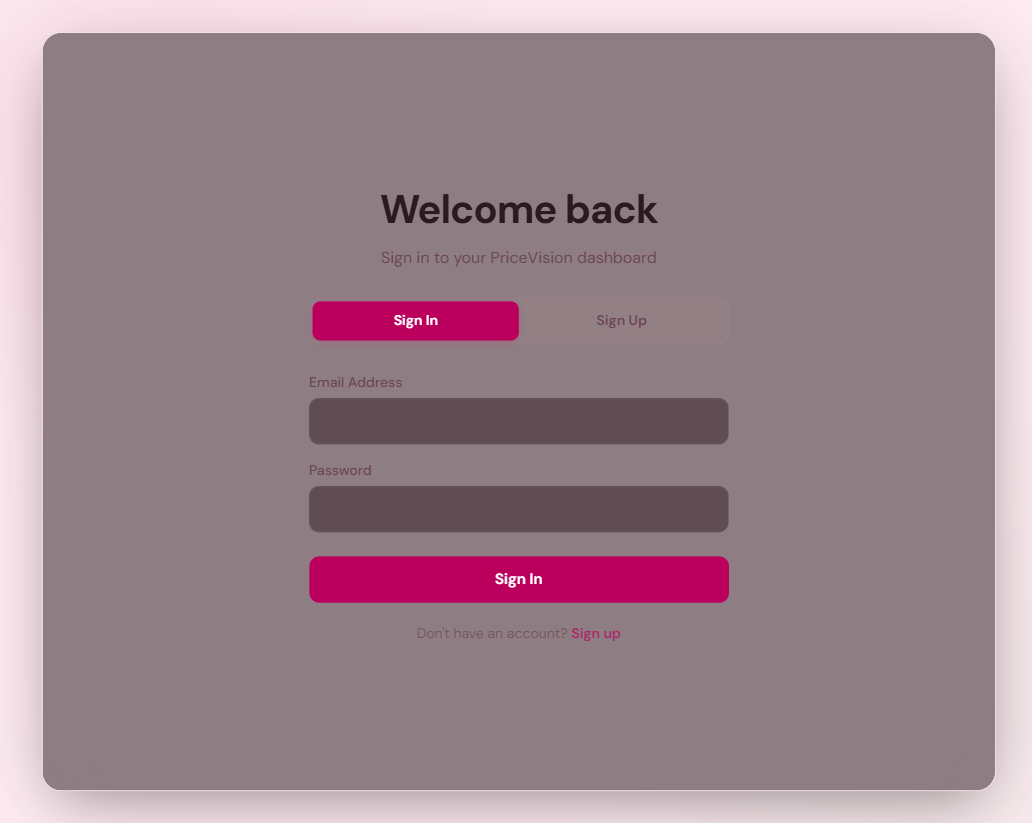
\includegraphics[width=0.88\textwidth]{auth-page.png}
}{
  \fbox{\parbox[c][6cm][c]{0.78\textwidth}{\centering Capture de l'ecran d'authentification non disponible.}}
}
\caption{Ecran d'authentification de la plateforme}
\label{fig:auth-screen}
\end{figure}

\section{Criteres de qualite de l'interface}
La qualite de l'interface ne se limite pas a l'esthetique. Les montants, les statuts et les changements doivent etre lisibles sans ambiguite. L'application applique un theme sombre par defaut, des composants accessibles et une navigation utilisable sur des ecrans de bureau et mobiles. React fournit un modele a composants et des hooks adaptes a la composition d'une interface interactive \cite{react}. La plateforme l'emploie avec un routeur client, des composants de formulaire et une couche de requetes typee.

\section*{Conclusion du chapitre}
Les specifications etablissent une chaine fonctionnelle allant de la connexion Shopify jusqu'a la recommandation. La suite du rapport precise l'architecture technique qui permet de realiser cette chaine de maniere modulaire et securisee.
\clearpage

% ==================== Chapitre 3 ====================
\chapter{Conception technique et architecture}
\section*{Introduction du chapitre}
Ce chapitre presente l'architecture par couches, le modele de donnees, le flux de surveillance et la logique de recommandation de prix.

\section{Architecture generale}
La solution adopte une architecture web de type client-serveur. Le client React affiche les vues metier et appelle l'API tRPC. Le serveur Express centralise les regles de securite, les routers, les services applicatifs et l'acces aux donnees. PostgreSQL conserve les donnees operationnelles et historiques. Des services externes interviennent pour Shopify et pour la collecte ou l'extraction des informations concurrentes.

\begin{figure}[H]
\centering
\begin{tikzpicture}[
  node distance=7mm and 8mm,
  layer/.style={draw=emsiBlue,rounded corners,fill=softBlue,align=center,minimum width=3.3cm,minimum height=1cm,font=\small},
  external/.style={draw=black!55,dashed,rounded corners,align=center,minimum width=2.65cm,minimum height=0.9cm,font=\small},
  arrow/.style={-{Stealth[length=2.1mm]},thick,draw=emsiBlue}
]
\node[layer] (client) {Client React + Vite\\Routes et tableau de bord};
\node[layer,right=of client] (api) {Serveur Express + tRPC\\Authentification et routers};
\node[layer,right=of api] (services) {Services metier\\Monitoring, alertes, recommandations};
\node[layer,below=of api] (db) {PostgreSQL + Drizzle ORM\\Donnees et historique};
\node[external,below=of client] (shopify) {Shopify\\OAuth et produits};
\node[external,below=of services] (external) {Recherche, scraping\\et extraction IA};
\draw[arrow] (client) -- node[above,font=\scriptsize]{tRPC sur HTTP} (api);
\draw[arrow] (api) -- (services);
\draw[arrow] (api) -- (db);
\draw[arrow] (api) |- (shopify);
\draw[arrow] (services) -- (external);
\draw[arrow] (services) |- (db);
\end{tikzpicture}
\caption{Architecture logique de Shopify Price Intelligence}
\label{fig:architecture}
\end{figure}

Cette separation permet de limiter les responsabilites de chaque couche. Le client n'a pas a manipuler les jetons Shopify ; l'API traite les actions authentifiees ; les services concentrent les traitements de domaine ; et le schema de donnees rend les relations explicites. Drizzle ORM permet de declarer un schema relationnel en TypeScript tout en conservant des operations proches de SQL \cite{drizzle}.

\section{Organisation du backend}
Le point d'entree configure les entetes de securite, la politique CORS, les limites de debit, les parseurs de requetes et les routes OAuth. Les routers tRPC exposent les domaines d'authentification, produits, concurrents, prix, alertes, recommandations, activite, intelligence, moteur de prix et Shopify. Chaque router delegue les operations lourdes aux services specialises.

\begin{table}[H]
\centering
\caption{Principaux modules serveur et leurs responsabilites}
\label{tab:server-modules}
\begin{tabularx}{\textwidth}{p{0.31\textwidth}Y}
\toprule
\textbf{Module} & \textbf{Responsabilite} \\
\midrule
\texttt{\_core/index.ts} & Demarrage Express, middleware de securite, SSE et planificateur. \\
\texttt{routers.ts} & Composition de l'API tRPC et operations de cycle de vie Shopify. \\
\texttt{services/product.service.ts} & Regles de creation, mise a jour, recherche et synchronisation des produits. \\
\texttt{services/price-monitoring.service.ts} & Collecte, extraction, instantanes, changements et alertes. \\
\texttt{services/pricing-engine.service.ts} & Calcul pur de moyenne, position de marche et prix recommande. \\
\texttt{\_core/auth/} & Sessions JWT, renouvellement, verification HMAC et chiffrement des jetons. \\
\bottomrule
\end{tabularx}
\end{table}

\section{Modele de donnees}
Le modele relationnel regroupe les entites de compte, d'integration, de catalogue et de surveillance. Un utilisateur peut posseder plusieurs boutiques ; une boutique contient des produits ; un produit peut etre associe a plusieurs produits concurrents ; chaque association produit des instantanes et, eventuellement, des changements. Les alertes et les journaux d'activite conservent une vue orientee utilisateur des evenements significatifs.

\begin{table}[H]
\centering
\caption{Entites de persistance principales}
\label{tab:data-model}
\begin{tabularx}{\textwidth}{p{0.25\textwidth}Y}
\toprule
\textbf{Entite} & \textbf{Role dans le systeme} \\
\midrule
\texttt{users}, \texttt{refresh\_tokens} & Identite, role, session et renouvellement d'acces. \\
\texttt{shopify\_stores} & Boutique connectee, etat d'activation, scopes et dernier horodatage de synchronisation. \\
\texttt{products} & Catalogue interne, prix, cout, reference, statut et suivi. \\
\texttt{competitors}, \texttt{competitor\_products} & Concurrents et offres associees aux produits internes. \\
\texttt{price\_snapshots}, \texttt{price\_changes} & Historique immuable des observations et changements detectes. \\
\texttt{alerts}, \texttt{activity\_logs} & Signalement utilisateur et trace d'activite. \\
\texttt{ai\_extractions}, \texttt{competitor\_discoveries} & Donnees d'extraction, confiance et candidats trouves. \\
\texttt{cron\_runs}, \texttt{scrape\_logs} & Suivi des executions planifiees et traces de collecte. \\
\bottomrule
\end{tabularx}
\end{table}

\section{Flux de monitoring}
Le monitoring traite les associations concurrent-produit actives. Pour chaque URL, le service tente de recuperer le contenu, enregistre un journal de collecte, appelle le module d'extraction et verifie le seuil de confiance. Lorsqu'une extraction est valide, un nouvel instantane est ajoute. La nouvelle valeur est ensuite comparee au prix precedent. Une variation produit un enregistrement de changement, un evenement d'activite et, si le seuil est atteint, une alerte diffusee au client via SSE.

\begin{figure}[H]
\centering
\begin{tikzpicture}[
  node distance=5mm,
  step/.style={draw=emsiBlue,rounded corners,fill=softBlue,align=center,minimum width=4.8cm,minimum height=0.8cm,font=\small},
  decision/.style={diamond,draw=emsiBlue,fill=softBlue,align=center,aspect=2.1,inner sep=1.5pt,font=\scriptsize},
  arrow/.style={-{Stealth[length=1.9mm]},thick,draw=emsiBlue}
]
\node[step] (start) {Selection des associations actives};
\node[step,below=of start] (scrape) {Collecte de la page concurrente et journalisation};
\node[decision,below=of scrape] (match) {Extraction validee\\et correspondance confirmee ?};
\node[step,below=of match] (snapshot) {Ajout d'un instantane et comparaison au precedent};
\node[decision,below=of snapshot] (change) {Variation detectee ?};
\node[step,below=of change] (alert) {Evenement, alerte et regeneration de recommandation};
\draw[arrow] (start) -- (scrape);
\draw[arrow] (scrape) -- (match);
\draw[arrow] (match) -- node[right,font=\scriptsize]{oui} (snapshot);
\draw[arrow] (snapshot) -- (change);
\draw[arrow] (change) -- node[right,font=\scriptsize]{oui} (alert);
\draw[arrow] (match.east) -- ++(2,0) node[above,font=\scriptsize]{non} |- (start.east);
\draw[arrow] (change.east) -- ++(2,0) node[above,font=\scriptsize]{non} |- (start.east);
\end{tikzpicture}
\caption{Sequence de surveillance et de detection des changements}
\label{fig:monitoring-flow}
\end{figure}

\section{Moteur de recommandation tarifaire}
Le moteur applique une regle explicable. Soit $P_c$ l'ensemble des prix concurrents valides, $\overline{P_c}$ leur moyenne, $C$ le cout du produit et $P_r$ le prix recommande. La moyenne est calculee apres exclusion des valeurs nulles, negatives ou egales a zero. Le prix cible de marche est obtenu par sous-cotation de 5\% :
\begin{equation}
P_{cible} = 0.95 \times \overline{P_c}
\label{eq:undercut}
\end{equation}

Lorsque le cout est connu et strictement positif, une protection de marge impose un plancher correspondant a 10\% au-dessus du cout :
\begin{equation}
P_{min} = 1.10 \times C
\label{eq:margin-floor}
\end{equation}
La recommandation finale est donc definie par l'equation \ref{eq:recommendation}.
\begin{equation}
P_r = \max(P_{cible}, P_{min})
\label{eq:recommendation}
\end{equation}

La position de marche est egalement classee. Une difference absolue inferieure ou egale a 3\% de la moyenne est consideree comme competitive. Un prix plus bas est classe comme leader de marche, tandis qu'un prix significativement superieur est considere comme surcote. En l'absence de prix concurrent valide, le systeme retourne un etat de donnees insuffisantes plutot qu'une recommandation artificielle.

\begin{table}[H]
\centering
\caption{Exemple de calcul d'une recommandation}
\label{tab:pricing-example}
\begin{tabularx}{\textwidth}{p{0.38\textwidth}Y}
\toprule
\textbf{Donnee} & \textbf{Valeur} \\
\midrule
Prix concurrents valides & 90,00 ; 100,00 ; 110,00 \\
Moyenne concurrentielle $\overline{P_c}$ & 100,00 \\
Prix cible selon l'equation \ref{eq:undercut} & 95,00 \\
Cout de revient $C$ & 90,00 \\
Plancher de marge selon l'equation \ref{eq:margin-floor} & 99,00 \\
Prix recommande $P_r$ & 99,00, avec protection de marge activee \\
\bottomrule
\end{tabularx}
\end{table}

\section{Conception de la securite}
La securite est integree des le serveur. Les sessions applicatives reposent sur des cookies HTTP-only contenant des JWT a duree limitee, completes par des jetons de renouvellement. Les mots de passe sont haches, les jetons Shopify sont chiffres au repos et ne sont pas exposes a l'interface cliente. La validation de domaine Shopify, les signatures HMAC, les limites de debit et la protection CSRF des routes OAuth constituent des controles complementaires. Les entetes HTTP sont renforces avec Helmet et les origines CORS sont restreintes en production.

Cette conception doit etre consideree comme une base technique qui exige une revue reguliere. Les proprietes de securite effectives dependent aussi de la configuration des secrets, des origines autorisees, des droits Shopify demandes et de l'observation des journaux de production.

\section*{Conclusion du chapitre}
La conception articule des responsabilites distinctes autour d'un historique de prix et d'un moteur de recommandation explicable. Le chapitre suivant decrit la traduction de cette conception en composants concrets et le protocole de validation associe.
\clearpage

% ==================== Chapitre 4 ====================
\chapter{Realisation et validation}
\section*{Introduction du chapitre}
Ce chapitre decrit les principaux choix d'implementation, les ecrans realises et la strategie de verification retenue pour le projet.

\section{Implementation du client web}
Le client est developpe avec React et Vite. Le point d'entree applique un garde d'authentification : tant que l'identite de l'utilisateur n'est pas disponible, une vue de chargement est affichee ; un utilisateur non authentifie est renvoye vers l'ecran de connexion. Les routes authentifiees sont placees dans une mise en page commune contenant la navigation laterale, la recherche, les alertes en temps reel, l'export CSV et l'acces aux principales fonctions.

La figure \ref{fig:products-screen} presente la page de gestion des produits disponible dans le projet. Cet ecran permet de visualiser un catalogue avant de le relier a des donnees concurrentielles.
\begin{figure}[H]
\centering
\IfFileExists{../products-page.png}{
  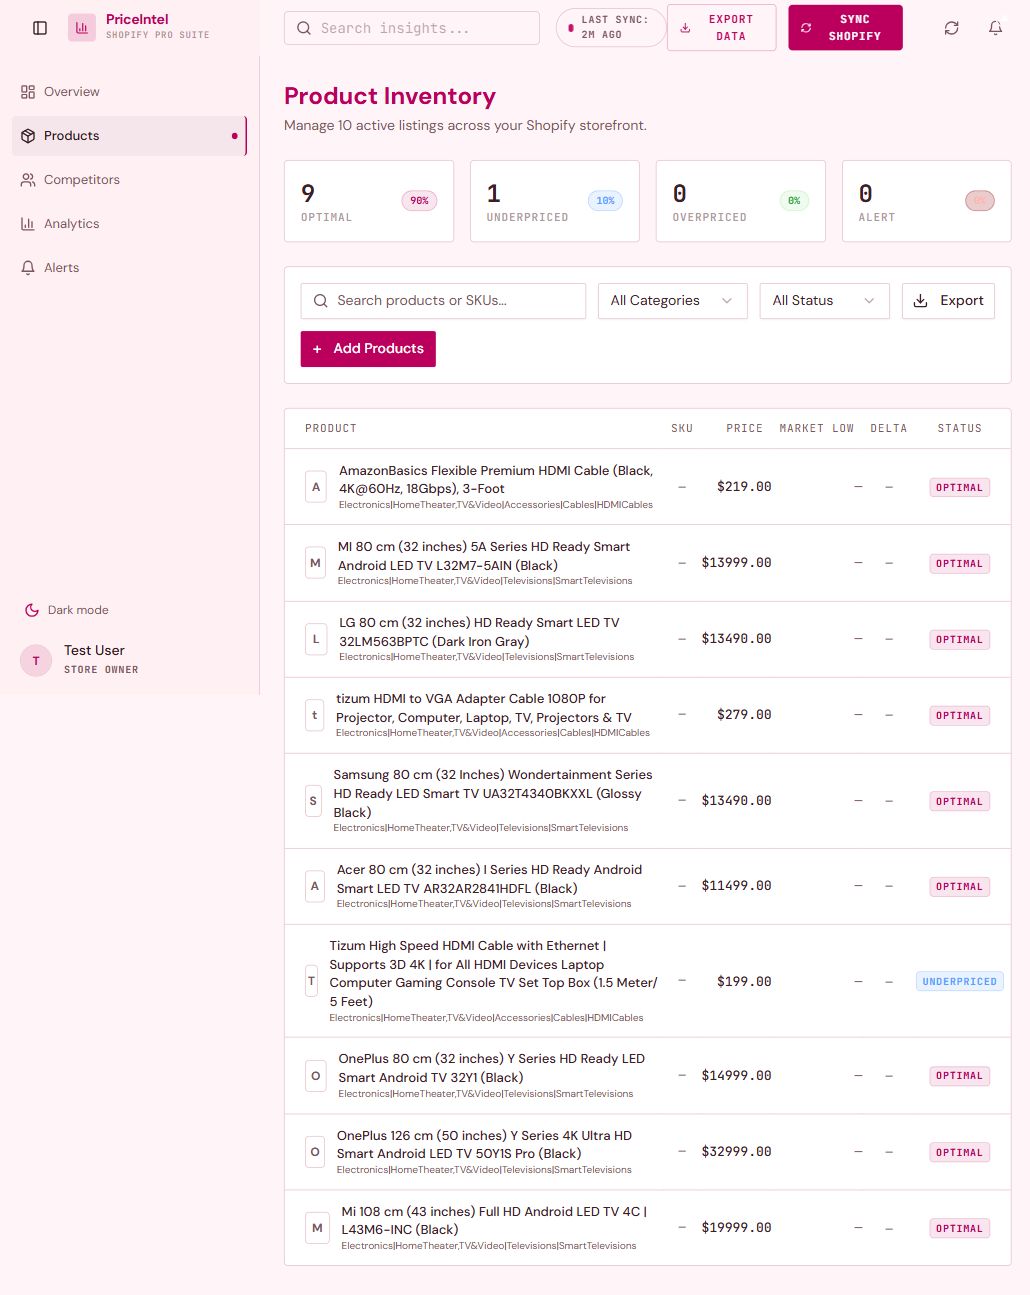
\includegraphics[width=0.93\textwidth]{products-page.png}
}{
  \fbox{\parbox[c][6cm][c]{0.78\textwidth}{\centering Capture de la page produits non disponible.}}
}
\caption{Page de gestion du catalogue produits}
\label{fig:products-screen}
\end{figure}

Les appels de donnees sont construits avec le client tRPC et React Query. Cette approche favorise la coevolution entre les contrats serveur et client : les parametres et les resultats des procedures sont types. Les composants de l'interface reutilisent des primitives accessibles afin de conserver une coherence visuelle entre les formulaires, tableaux, dialogues et notifications.

\section{Implementation de l'API et des services}
Le serveur est une application Express executee en TypeScript. La couche tRPC transporte les procedures metier et applique des procedures publiques ou protegees selon le domaine. Les routes Shopify permettent l'echange de code OAuth, l'enregistrement d'une boutique, la deconnexion et la synchronisation paginee des produits. Les operations de synchronisation verifient l'appartenance de la boutique a l'utilisateur courant avant d'acceder au jeton stocke.

Le service de monitoring suit une sequence de traitement prevue pour etre observable : creation d'une execution de planification, collecte, journalisation, extraction, creation d'instantane, mise a jour de l'offre concurrente, detection de changement et diffusion de notification. En cas d'erreur sur une offre, l'erreur est enregistree et le traitement des autres offres peut continuer. Cette granularite facilite le diagnostic des problemes provenant d'une URL ou d'un connecteur externe.

\section{Extrait de logique tarifaire}
La logique suivante illustre le caractere deterministe du calcul. Le code de production isole cette logique dans un module sans acces reseau ni base de donnees, ce qui facilite les tests unitaires.
\begin{lstlisting}[style=typescript,caption={Pseudo-code simplifie de la protection de marge},label={lst:pricing}]
const targetPrice = averageCompetitorPrice * 0.95;

if (costPrice == null || costPrice <= 0) {
  return targetPrice;
}

const minimumAllowedPrice = costPrice * 1.10;
return Math.max(targetPrice, minimumAllowedPrice);
\end{lstlisting}

L'algorithme de la liste \ref{lst:pricing} ne remplace pas une politique commerciale complete. Il fournit une regle de depart transparente, dont les parametres de sous-cotation et de marge peuvent etre rendus configurables dans une evolution ulterieure.

\section{Jeu de tests et protocole de validation}
Le depot contient des tests unitaires pour le moteur de prix et des tests d'integration relatifs aux produits et a la deconnexion. Les tests du moteur couvrent notamment la moyenne de prix valides, le filtrage de valeurs invalides, l'absence de donnees, la sous-cotation de 5\%, la protection de marge, les seuils de classification et les cas limites. Les tests de produits verifient des regles de creation, de normalisation de reference, d'unicite par utilisateur, de recherche et de retrocompatibilite.

Le tableau \ref{tab:validation-protocol} fournit un protocole reproductible. Les resultats chiffres et les captures de la campagne finale doivent etre renseignes apres execution dans l'environnement de soutenance. Cette precaution evite d'affirmer des resultats qui ne sont pas directement observes.

\begin{table}[H]
\centering
\caption{Protocole de validation a executer avant soutenance}
\label{tab:validation-protocol}
\begin{tabularx}{\textwidth}{p{0.16\textwidth}p{0.28\textwidth}Y}
\toprule
\textbf{Type} & \textbf{Scenario} & \textbf{Verification attendue} \\
\midrule
Unitaire & Moyenne de trois prix valides. & La moyenne est exacte et arrondie a deux decimales. \\
Unitaire & Prix cible inferieur au plancher de marge. & Le prix retourne est le plancher et le marqueur de protection est actif. \\
Integration & Creation de deux produits avec la meme reference pour un utilisateur. & La seconde creation est rejetee ; la meme reference reste possible pour un autre utilisateur. \\
Integration & Deconnexion d'une boutique Shopify. & La boutique ciblee devient inactive et le jeton est retire. \\
Fonctionnel & Connexion, synchronisation et affichage du catalogue. & Les produits lies a la boutique sont visibles uniquement pour le marchand concerne. \\
Fonctionnel & Variation d'un prix concurrent superieure au seuil. & Un instantane, un changement, une activite et une alerte sont crees. \\
Securite & Acces a une ressource appartenant a un autre compte. & La requete est refusee ou ne retourne aucune donnee etrangere. \\
\bottomrule
\end{tabularx}
\end{table}

\section{Commandes de verification}
Les commandes suivantes sont definies dans le manifeste du projet. Elles doivent etre executees une a une dans un environnement configure avec les variables necessaires et une base de donnees de test. La sortie exacte, la date d'execution et les anomalies rencontrees doivent etre ajoutees dans l'annexe de la version soumise.
\begin{lstlisting}[style=typescript,caption={Commandes de verification du projet}]
pnpm check
pnpm test
pnpm build
\end{lstlisting}

\section{Contraintes observees et ameliorations}
La qualite des recommandations depend des donnees collectees. Les pages concurrentes peuvent changer de structure, devenir inaccessibles ou proposer des variantes ambigues. Il est donc pertinent de conserver la confiance de l'extraction, la source et la date de l'observation. Le traitement planifie en processus unique convient a une premiere version mais devra evoluer vers une file de travaux et des executeurs distribues lorsque le volume de produits augmentera.

Les ameliorations prioritaires sont les suivantes :
\begin{itemize}
  \item rendre les regles de recommandation configurables par categorie ou par strategie commerciale ;
  \item ajouter une validation humaine simple pour les rapprochements ambigus ;
  \item isoler les taches de scraping dans une file de travaux avec reprise et observation centralisee ;
  \item enrichir les indicateurs de tendance par periode et par concurrent ;
  \item ajouter une campagne de tests de securite et de charge documentee avant la mise en production.
\end{itemize}

\section*{Conclusion du chapitre}
La realisation transforme la conception en une application modulaire couvrant les principaux flux metier. Les tests existants constituent une base de verification ; leur execution tracee et une campagne de validation complete sont necessaires avant toute conclusion quantitative de production.
\clearpage

% ==================== Conclusion ====================
\chapter*{Conclusion generale et perspectives}
\addcontentsline{toc}{chapter}{Conclusion generale et perspectives}
\markboth{Conclusion generale et perspectives}{Conclusion generale et perspectives}

Ce projet avait pour objectif de concevoir et de realiser une plateforme d'intelligence tarifaire pour les marchands Shopify. La solution proposee centralise le catalogue, les offres concurrentes, les instantanes de prix, les changements detectes et les recommandations. Elle repond au besoin initial de reduire la surveillance manuelle en organisant une chaine allant de la connexion de la boutique jusqu'a l'alerte ou a la decision tarifaire.

Les contributions principales sont une architecture TypeScript par couches, une modelisation relationnelle orientee historique, un flux de monitoring trace, une interface de tableau de bord et un moteur de recommandation explicable. La regle de calcul combine une position de marche avec une protection de marge, ce qui evite de presenter la baisse de prix comme une decision automatique et universelle. La securite est prise en compte par l'authentification, le chiffrement des jetons sensibles, les limites de debit, la protection CSRF et la separation des donnees utilisateurs.

Les perspectives concernent principalement le passage a l'echelle et l'enrichissement de la decision. Une file de travaux distribuee, des politiques de prix parametrables, une validation humaine des rapprochements, des indicateurs de tendance et une campagne de tests de performance permettraient de faire evoluer la solution vers une exploitation plus large. Avant le deploiement en production, les resultats du protocole de validation, les captures finales et les informations academiques devront etre completes et verifies.

% ==================== References ====================
\clearpage
\addcontentsline{toc}{chapter}{References bibliographiques}
\bibliographystyle{IEEEtran}
\bibliography{references}

% ==================== Annexes ====================
\appendix
\chapter{Trace de conformite au guide EMSI}
\begin{longtable}{p{0.34\textwidth}p{0.56\textwidth}}
\toprule
\textbf{Exigence du guide} & \textbf{Application dans ce rapport} \\
\midrule
\endhead
Classe A4 et marges 2,5 / 2,5 / 3 / 2,5 cm & Classe \texttt{report} et paquet \texttt{geometry} configures dans le preambule. \\
Texte 12 pt et interligne 1,5 & Classe 12 pt et commande \texttt{\string\onehalfspacing}. \\
Pages preliminaires romaines puis contenu arabe & Commandes \texttt{\string\pagenumbering\{roman\}} et \texttt{\string\pagenumbering\{arabic\}}. \\
Page de garde & Presente avec emplacements pour logos, filiere, encadrements, entreprise et annee. \\
Resume, abstract et ملخص & Trois sections independantes, suivies de mots-cles en francais et anglais. \\
Tables et listes automatiques & Table des matieres, liste des figures et liste des tableaux. \\
Structure des chapitres & Chaque chapitre contient une introduction et une conclusion. \\
Figures, tableaux et equations & Figures et tableaux numerotes avec legendes ; equations \ref{eq:undercut} a \ref{eq:recommendation}. \\
Bibliographie & Citations numeriques et fichier BibTeX \texttt{references.bib}. \\
\bottomrule
\end{longtable}

\chapter{Checklist de finalisation avant impression}
\begin{enumerate}
  \item Remplacer tous les textes rouges entre crochets par les informations reelles.
  \item Inserer les logos officiels et, si necessaire, ajuster leur taille.
  \item Verifier les trois resumes avec les encadrants et la filiere.
  \item Executer les tests, conserver les resultats et completer le tableau de validation.
  \item Ajouter les captures finales de l'application et verifier les legendes.
  \item Verifier que chaque information externe est citee et que les dates de consultation sont a jour.
  \item Compiler avec LuaLaTeX et BibTeX jusqu'a stabilisation de la table des matieres et des references.
  \item Relire orthographe, grammaire, pagination, alignement et impression PDF.
\end{enumerate}

\chapter{Exemple de donnees de test tarifaires}
\begin{table}[H]
\centering
\caption{Jeu de donnees illustratif pour tester le moteur de prix}
\begin{tabular}{lrrrr}
\toprule
Produit & Cout & Prix marchand & Moyenne concurrents & Prix recommande \\
\midrule
Cas A & 50,00 & 105,00 & 100,00 & 95,00 \\
Cas B & 90,00 & 105,00 & 100,00 & 99,00 \\
Cas C & Non renseigne & 100,00 & 100,00 & 95,00 \\
Cas D & 80,00 & 100,00 & Non disponible & Non disponible \\
\bottomrule
\end{tabular}
\end{table}

\end{document}
